%************************************************
\chapter{Multiway Structural Entropic Distance}\label{ch:msed}
%************************************************
%\begin{flushleft}{\slshape    
%    At the time, Nixon was normalizing relations with China.  
%    I figured that if he could normalize relations, then so could I} \\ \medskip
%    --- Edgar Codd
%\end{flushleft}
%
Much of the research on similarity search focuses on the similarity (or distance) between two objects.  For many situations, however, ascertaining the mutual similarity of a set of objects would be useful. Applications could be, for example, similarity joins, clustering, cluster analysis, and potentially many more that are dependent upon these techniques.

The calculation of density, or multi-way divergence as the analogue to distance, has been rarely used and is typically calculated through some compound function over the set of pair-wise distances within the set of objects: for example, the mean inter-set distance or the mean distance from each object to a centroid.  
%If the divergence function is used frequently, a large number of calls may be required of the, typically expensive, distance metric, making this type of operation prohibitively expensive.

In this chapter, we derive a function to calculate the divergence of a set of objects that is based on the structural entropic distance discussed in chapter \ref{ch:sim_structured_data}.  This new metric, which is grounded in information theory, avoids the problem of repeated calls to the distance metric through a direct, calculable notion of multi-way divergence without relying on approximation.  It reuses the notion of complexity offered in the definition of the original distance metric and reverts to this definition when the size of the set is two.  It is bounded, giving a maximum value when there is no commonality, allowing absolute comparisons to be made.  And finally, it is only a little more expensive than a single distance to evaluate.

We show that multi-way divergence offers a cheaper alternative to compound functions whilst giving similar, or better, semantic properties.  We believe it could be applied usefully to construct new metric indices or to execute more complex queries, such as similarity joins, efficiently. 
\section{Multiway distances}
The notion of a multi-way distance metric is not new,  motivation coming from geometry and topology.  Recently a few papers have  analysed the generalisation to multi-way for any existing metric\cite{Warrens2009, Warrens2010, Deza2000797}.  They consider whether various axioms are observed in these generalisations. For example, a metric space with a simple dyadic metric has the following axioms:
%
\begin{equation*}
\begin{aligned}
    d(x, y) &= 0 \Leftrightarrow x = y \\
    d(x, y) &= d(y, x) \\
    d(x, y) &\leq d(x, z) + d(y, z)
\end{aligned}
\end{equation*}
%
The first of these, is simply generalised to $D(x_1, \ldots, x_n) = 0$ if and only if all $x_i$ are equal; the second to $D(x_{\pi(1)}, \ldots, x_{\pi(n)}) = D(x_1, \ldots, x_n)$ for every permutation $\pi$ of $\{1, 2, \ldots, n\}$; while the third, triangle inequality, has been generalised in numerous ways\cite{Warrens2010}, such as polyhedron inequality:
%
\begin{equation*}
    (n - 1) \cdot D(x_1, \ldots, x_n) \leq \sum_{i = 1}^n D(x_1, \ldots, x_{i-1}, x_{i + 1},\ldots, x_{n+1})
\end{equation*}
%

These generalised axioms are interesting in their own right, and the first two  are desirable properties of a multi-way divergence function, but it is not clear if polyhedron inequality aids similarity search at this stage.
\subsection{Compound metrics} 
Deza and Rosenberg introduced the multi-way extension of the star distance in \cite{Deza2000797}, while perimeter distance\cite{Warrens2010} gives a geometrical ``average distance''.  Both of these, however, are compound functions and do not fundamentally look at generalising any specific metric.


\subsection{Multiway structural entropic distance (MSED)}

Let $X_1, \ldots X_n$ be the sources emitting the streams $E_1, \ldots E_n$; let $Y$ be the notional source emitting the merged stream $F = \{f_1, f_2, \ldots, f_m\}$ where $\forall E_i,  E_i \subseteq F$, then  
\begin{equation}
	P_Y(f_i) = \frac{\sum_{j=1}^n P_{X_j}(f_i)}{n}
\end{equation}
Recall from chapter \ref{ch:sim_structured_data} that the complexity of a source $X_i$ is given by the logarithmic base $b$ raised to the power of the entropy $H_b(X_i) = -\sum_{e \in E_i} P_{X_i}(e) \log_b P_{X_i}(e)$ of that source, $C(X_i) = b^{H_b(X_i)}$.  

Using the same principle as before of applying the ratio of the complexity of the merged stream to the geometric mean of individual complexities, we arrive at the ratio 
\begin{equation}
\frac{C(Y)}{\sqrt[n]{\prod_{i=1}^n C(X_i)}}
\end{equation}
which gives a value in the range $[1, n]$; we scale this to $[0,1]$ to give the multiway structural entropic distance:

\begin{equation}
MSED(X_1, \ldots X_n) = \frac{1}{n - 1} \cdot \left(\frac{C(Y)}{\sqrt[n]{\prod_{i=1}^n C(X_i)}} - 1\right)
\end{equation}

As it should, the joint complexity equals the individual complexities when all structures are identical, and equals the sum of the individual
complexities when there is no common structure.

Using the same mapping to vector spaces as before, this generalised function remains a ratio of the complexity of a centroid to the geometric mean of its neighbours' complexities, and has the following properties:  
\begin{itemize}
\item If all vectors are identical it gives 0
\item If all vectors are different it gives 1
\item All other inputs give a value between these bounds
\end{itemize}

Consider now the metric space axioms described at the beginning of this section; we have stated that the lower bound is achieved when all elements are the same, so the first axiom holds.  Since all operations involved in both the numerator and denominator are associative, total symmetry holds too. We do not yet know whether polyhedron inequality holds. 
\subsection{Relationship to Jensen-Shannon divergence}
As we saw in the last chapter, SED is related to Jensen-Shannon.  A similar relationship exists between the two multi-way versions.  Recall that Jensen-Shannon may be expressed in vector notation as:
\begin{equation}
JSD(\mathbf{x}, \mathbf{y}) = H_b(\frac{1}{2} (\mathbf{x} + \mathbf{y})) - \frac{1}{2}(H_b(\mathbf{x}) + H_b(\mathbf{y}))
\end{equation}

When defining Jensen-Shannon divergence, Lin\cite{} also described a multi-way generalisation:
\begin{equation}
JSD(\mathbf{x^{(1)}},\ldots, \mathbf{x^{(n)}}) = H_b(\frac{1}{n}\sum_{i = 1}^n \mathbf{x^{(i)}}) - \frac{1}{n} \sum_{i = 1}^n H_b(\mathbf{x^{(i)}})
\end{equation}
\begin{mytheorem}{$MSED(\mathbf{x^{(1)}},\ldots, \mathbf{x^{(n)}}) = \frac{b^{JSD(\mathbf{x^{(1)}},\ldots, \mathbf{x^{(n)}})} - 1}{n - 1}$}
\begin{proof}\label{proof:JS}
\begin{align}
MSED(\mathbf{x^{(1)}},\ldots, \mathbf{x^{(n)}}) &= \frac{1}{n - 1} \cdot \left(\frac{C(\frac{1}{n}\sum_{i = 1}^n \mathbf{x^{(i)}})}{\sqrt[n]{\prod_{i=1}^n \strut C(\mathbf{x^{(i)}})}} - 1\right)\\
&= \frac{1}{n - 1} \cdot \left(\frac{b^{H_b(\frac{1}{n}\sum_{i = 1}^n \mathbf{x^{(i)}})}}{\sqrt[n]{\prod_{i=1}^n \strut b^{H_b(\mathbf{x^{(i)}})}}} - 1\right)\\
&= \frac{1}{n - 1} \cdot \left(\frac{b^{H_b(\frac{1}{n}\sum_{i = 1}^n \mathbf{x^{(i)}})}}{b^{\frac{1}{n} \sum_{i=1}^n H_b(\mathbf{x^{(i)}})}} - 1\right)\\
%
&= \frac{1}{n - 1} \cdot (b^{H_b(\frac{1}{n}\sum_{i = 1}^n \mathbf{x^{(i)}}) -\frac{1}{n}\sum_{i=1}^n H_b(\mathbf{x^{(i)}})} - 1)\\
&= \frac{b^{JSD(\mathbf{x^{(1)}},\ldots, \mathbf{x^{(n)}})} - 1}{n - 1}
\end{align}
\end{proof}
\end{mytheorem}

%\subsection{old-Generalisation}
%Consider the algebraic rewrite of SED introduced in chapter 3 which culminates with final equation:
%
%\begin{myMaths}
%d(X,Y) = 2 \cdot \left( \prod_{e \in X \cap Y} 
%\left(u_e^{u_e} \cdot v_e^{v_e} \right)^{w}\right) - 1
%\end{myMaths}
%
%The product term itself is composed of three elements -- $u_e$, $v_e$, and $w_e$. $u_e$ and $v_e$ can be thought of themselves as relative frequencies of the particular frequency of term $e$, and $u_e + v_e = 1$. While $w_e$ is the mean of the relative frequencies of $e$.  
%
%With these two points in mind, the formula generalises to more than two variables (i.e. $d(X_1, \ldots, X_n)$) as follows.  First, since $u_e$ and $v_e$ may be thought of as relative frequencies, replace these with $u_{ie} = \frac{f_{X_i}(e)}  {\sum_{X} f_{X}(e)}$.  Then likewise with $w_e$, the mean, replace with $w_e = \frac{\sum_{X} f_{X}(e)}{n}$.  Now the product term can be written as
%
%\begin{myMaths}  
%\prod_{e \in \bigcap X}  \prod_{i = 1}^{n} u_{ie}^{u_{ie}w_e}   
%\end{myMaths}
%Next, notice that this product term is now in the range $[\frac{1}{n}, 1]$ and thus requires scaling to the range $[0,1]$ as before, giving the generalised multivariate distance function:
%
%\begin{myMaths} d(X_1, \ldots, X_n) = \frac{n \cdot \left(\prod_{e \in \bigcap X}  \prod_{i = 1}^{n} u_{ie}^{u_{ie}w_e}\right) - 1 }{n - 1}
%\end{myMaths}

\section{Correlations}
\begin{figure}
        \centering
        \subfloat[triples with mean structural entropic distance]{
				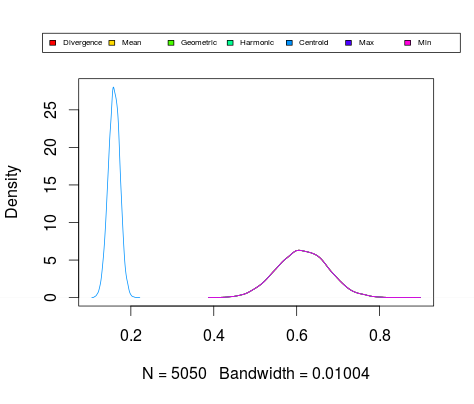
\includegraphics[width=0.5\textwidth]{gfx/correlations/2.png}
                \label{fig:triples}
        }%
        ~ %add desired spacing between images, e. g. ~, \quad, \qquad etc.
          %(or a blank line to force the subfigure onto a new line)
        \subfloat[5-tuples with mean euclidean distance to a centroid]{
                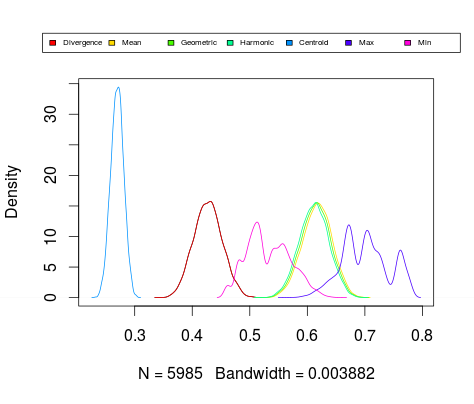
\includegraphics[width=0.5\textwidth]{gfx/correlations/4.png}
                \label{fig:5-tuples}
        }
        
        \subfloat[5-tuples with mean euclidean distance to a centroid]{
                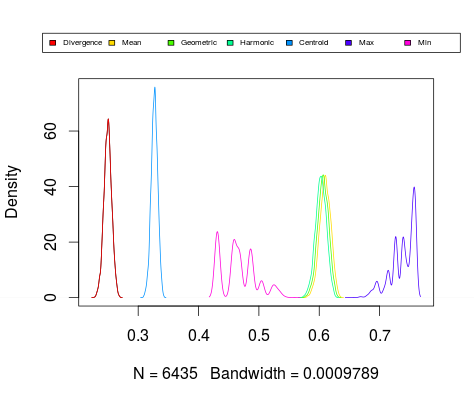
\includegraphics[width=0.5\textwidth]{gfx/correlations/8.png}
                \label{fig:5-tuples}
        }
        ~
        \subfloat[5-tuples with mean euclidean distance to a centroid]{
                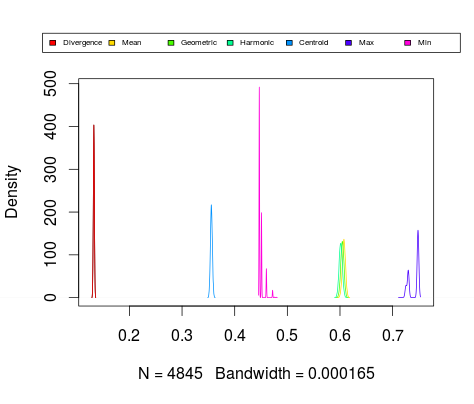
\includegraphics[width=0.5\textwidth]{gfx/correlations/16.png}
                \label{fig:5-tuples}
        }

        \caption[Correlation with divergence in 15-dimensional space]{Correlation with divergence in 15-dimensional space}\label{fig:corr-mean}
\end{figure}
%We compared our function to three other measures of multi-way divergence, based both on the SED metric and also on Euclidean distance. Set sizes of 3, 4 and 5 were chosen over randomly generated 5 and 15 dimensional probability vectors.  
%\begin{table}
% 
%\centering
%\begin{tabularx}{0.95\linewidth}{X l l l}
%\toprule
%\multicolumn{3}{r}{PCC} \\
%\cmidrule(r){2-4}
%5 dimension Structural entropic distance	& 3-tuple 	& 4-tuple 	& 5-tuple\\
%\midrule
%mean intra-cluster distance		& 0.991285		& 0.9918386		& 0.9943856\\
%mean distance to a centroid		& 0.9950909		& 0.9952373		& 0.9959319\\
%max intra-cluster distance		& 0.9365853		& 0.9027764		& 0.9021573\\	
%\midrule
%\multicolumn{3}{l}{5 dimension Euclidean distance} \\
%\midrule
%mean intra-cluster distance		& 0.9482936		& 0.9584011		& 0.9669735\\
%mean distance to a centroid		& 0.9478603		& 0.9565286		& 0.9634166\\
%max intra-cluster distance		& 0.9059921		& 0.8853846		& 0.8865668\\	
%\midrule
%\multicolumn{3}{l}{15 dimension Structural entropic distance} \\
%\midrule
%mean intra-cluster distance		& 0.9924866		& 0.990572		& 0.9915913\\
%mean distance to a centroid		& 0.9958805		& 0.9950946		& 0.9956354\\
%max intra-cluster distance		& 0.9166376		& 0.854482		& 0.8198081\\	
%\midrule
%\multicolumn{3}{l}{15 dimension Euclidean distance} \\
%\midrule
%mean intra-cluster distance		& 0.9645352		& 0.9657067		& 0.9677485\\
%mean distance to a centroid		& 0.964599		& 0.9649238		& 0.9662083\\
%max intra-cluster distance		& 0.8966909		& 0.8426229		& 0.8024388\\	
%\bottomrule
%\end{tabularx}
%\caption{Pearson's correlation coefficients for multi-way divergence}
%\label{term_table}
%\end{table}%
%The maximum distance within each cluster is taken by running through all pair-wise combinations and selecting the largest.  

The best correlation comes with the mean distance to a centroid.  This method is calculated by making a centroid using the mean vector then averaging all distances in the cluster to it.  Since multi-way divergence is a ratio of the complexity of a centroid to the geometric mean of individual complexities, there is much more in common with this definition.  Even when the comparison distance metric is Euclidean distance, a very strong correlation exists (figure \ref{fig:5-tuples}).

The mean intra-cluster distance also correlates well with multi-way divergence.  Figure \ref{fig:triples} shows the correlation with the mean intra-cluster distance, which appears to be strongest at the, more commonly used, lower end.  

Multi-way divergence correlates --  less strongly than the other methods -- with both SED and Euclidean maximum intra-cluster distance, and the correlation drops as the cluster size increases.  Rather than assessing the mutual similarity, the maximum distance simply describes the two farthest points in the cluster.  These two points must lie on the cluster perimeter and describe the spread of points across the space. Using only two points, however, fails to account for the spread in other dimensions, further verified by the drop in correlation in the higher dimensional space.
%\begin{figure}
%        \centering
%        \begin{subfigure}[b]{0.3\textwidth}
%                \centering
%				\includegraphics[width=\textwidth]{images/triples-max.png}
%                \caption{triples}
%                \label{fig:triples}
%        \end{subfigure}%
%        ~ %add desired spacing between images, e. g. ~, \quad, \qquad etc.
%          %(or a blank line to force the subfigure onto a new line)
%        \begin{subfigure}[b]{0.3\textwidth}
%                \centering
%                \includegraphics[width=\textwidth]{images/4-tuples-max.png}
%                \caption{4-tuples}
%                \label{fig:4-tuples}
%        \end{subfigure}
%        ~ %add desired spacing between images, e. g. ~, \quad, \qquad etc.
%          %(or a blank line to force the subfigure onto a new line)
%        \begin{subfigure}[b]{0.3\textwidth}
%                \centering
%                \includegraphics[width=\textwidth]{images/5-tuples-max.png}
%                \caption{5-tuples}
%                \label{fig:5-tuples}
%        \end{subfigure}
%        \caption{Correlations with maximum inter-cluster distance joining 15-dimensional spaces}\label{fig:corr-max}
%\end{figure}
\begin{figure}
        \centering
        \subfloat[triples with mean structural entropic distance]{
				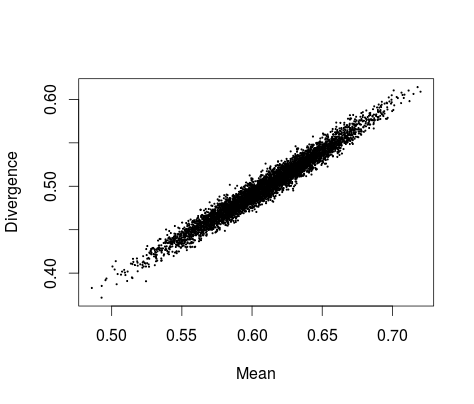
\includegraphics[width=0.5\textwidth]{gfx/correlations/3_mean.png}
                \label{fig:triples}
        }%
        ~ %add desired spacing between images, e. g. ~, \quad, \qquad etc.
          %(or a blank line to force the subfigure onto a new line)
        \subfloat[5-tuples with mean euclidean distance to a centroid]{
                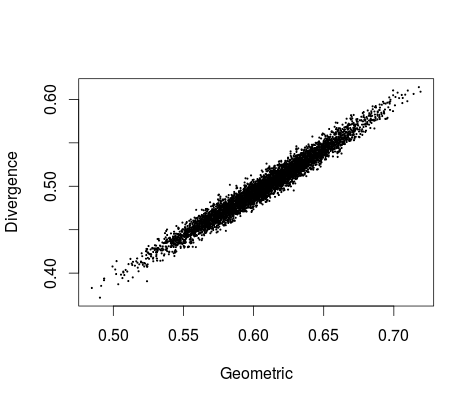
\includegraphics[width=0.5\textwidth]{gfx/correlations/3_geometric.png}
                \label{fig:5-tuples}
        }
        
        \subfloat[5-tuples with mean euclidean distance to a centroid]{
                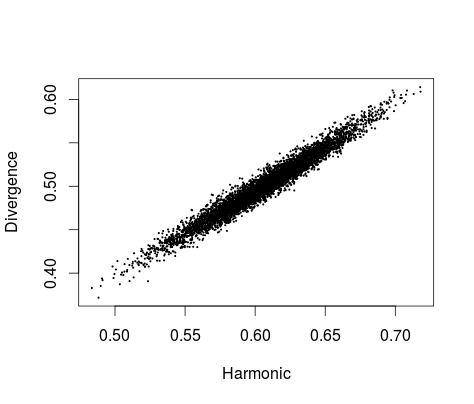
\includegraphics[width=0.5\textwidth]{gfx/correlations/3_harmonic.png}
                \label{fig:5-tuples}
        }
        ~
        \subfloat[5-tuples with mean euclidean distance to a centroid]{
                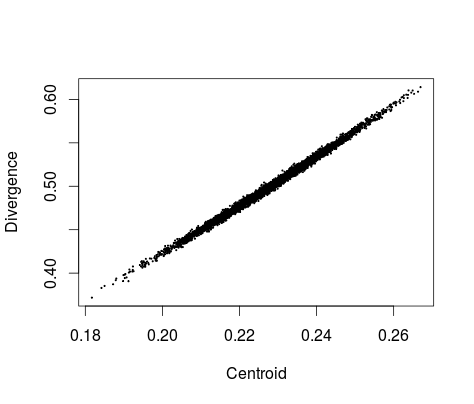
\includegraphics[width=0.5\textwidth]{gfx/correlations/3_centroid.png}
                \label{fig:5-tuples}
        }
                
        \subfloat[5-tuples with mean euclidean distance to a centroid]{
                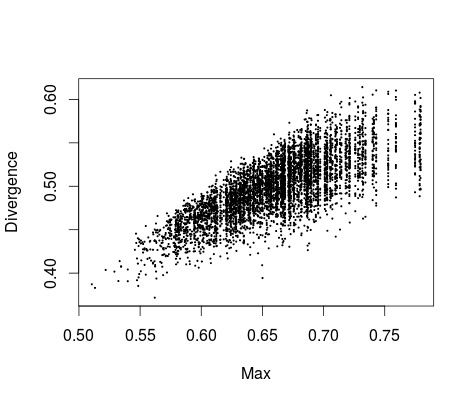
\includegraphics[width=0.5\textwidth]{gfx/correlations/3_max.png}
                \label{fig:5-tuples}
        }
        ~
        \subfloat[5-tuples with mean euclidean distance to a centroid]{
                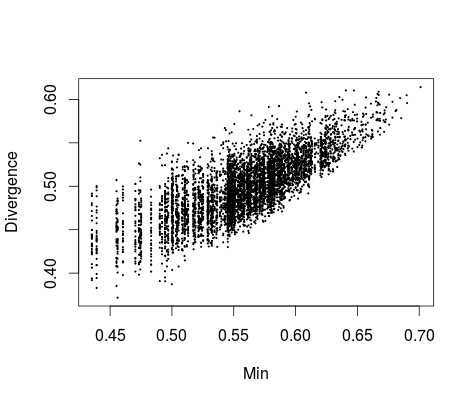
\includegraphics[width=0.5\textwidth]{gfx/correlations/3_min.png}
                \label{fig:5-tuples}
        }

        \caption[Correlation with divergence in 15-dimensional space]{Correlation with divergence in 15-dimensional space}\label{fig:corr-mean}
\end{figure}

\begin{figure}
        \centering
        \subfloat[triples with mean structural entropic distance]{
				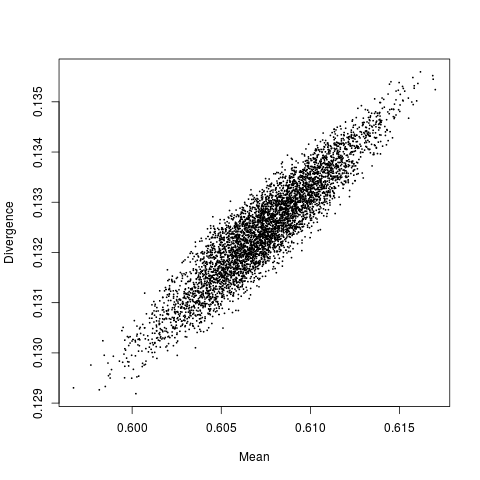
\includegraphics[width=0.5\textwidth]{gfx/correlations/16_Mean.png}
                \label{fig:triples}
        }%
        ~ %add desired spacing between images, e. g. ~, \quad, \qquad etc.
          %(or a blank line to force the subfigure onto a new line)
        \subfloat[5-tuples with mean euclidean distance to a centroid]{
                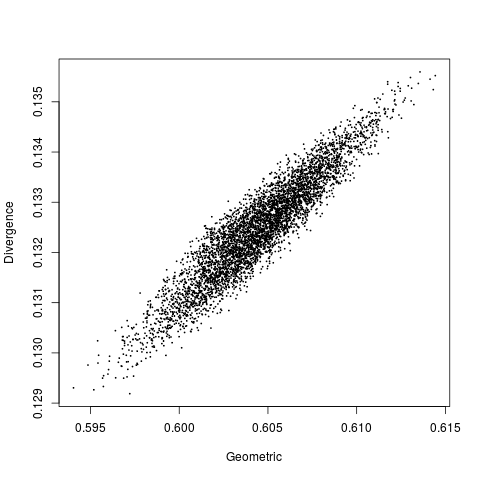
\includegraphics[width=0.5\textwidth]{gfx/correlations/16_Geometric.png}
                \label{fig:5-tuples}
        }
        
        \subfloat[5-tuples with mean euclidean distance to a centroid]{
                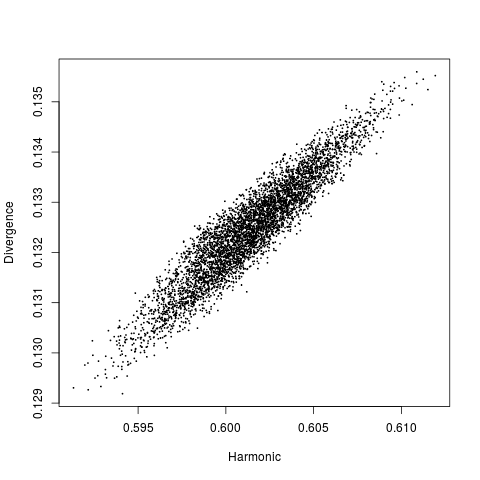
\includegraphics[width=0.5\textwidth]{gfx/correlations/16_Harmonic.png}
                \label{fig:5-tuples}
        }
        ~
        \subfloat[5-tuples with mean euclidean distance to a centroid]{
                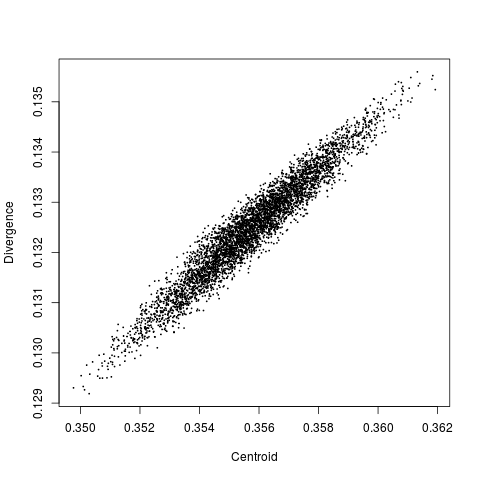
\includegraphics[width=0.5\textwidth]{gfx/correlations/16_Centroid.png}
                \label{fig:5-tuples}
        }
                
        \subfloat[5-tuples with mean euclidean distance to a centroid]{
                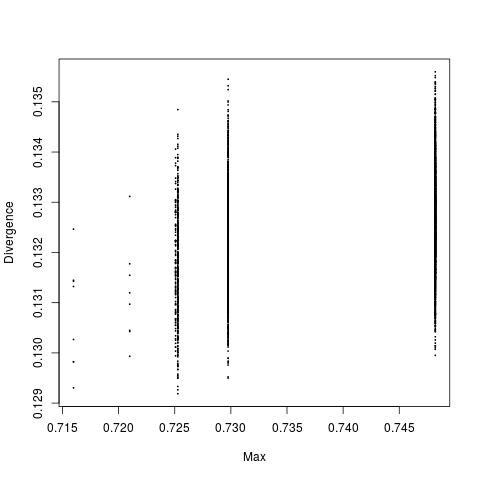
\includegraphics[width=0.5\textwidth]{gfx/correlations/16_Max.png}
                \label{fig:5-tuples}
        }
        ~
        \subfloat[5-tuples with mean euclidean distance to a centroid]{
                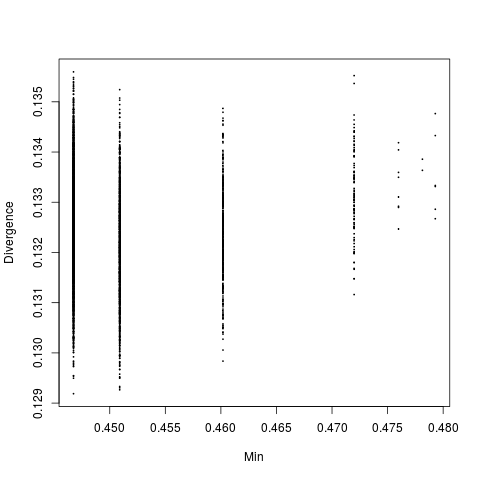
\includegraphics[width=0.5\textwidth]{gfx/correlations/16_Min.png}
                \label{fig:5-tuples}
        }

        \caption[Correlation with divergence in 15-dimensional space]{Correlation with divergence in 15-dimensional space}\label{fig:corr-mean}
\end{figure}

\begin{figure}
        \centering
        \subfloat[triples with mean structural entropic distance]{
				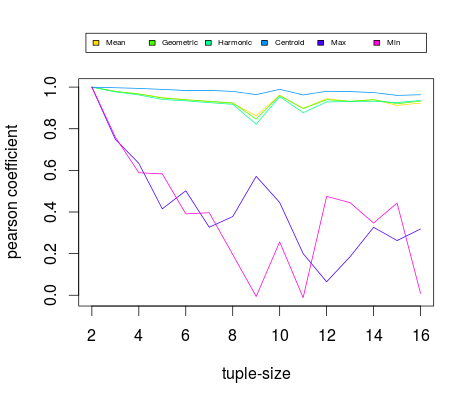
\includegraphics[width=0.5\textwidth]{gfx/correlations/pearson.png}
                \label{fig:triples}
        }%
        ~ %add desired spacing between images, e. g. ~, \quad, \qquad etc.
          %(or a blank line to force the subfigure onto a new line)
        \subfloat[5-tuples with mean euclidean distance to a centroid]{
                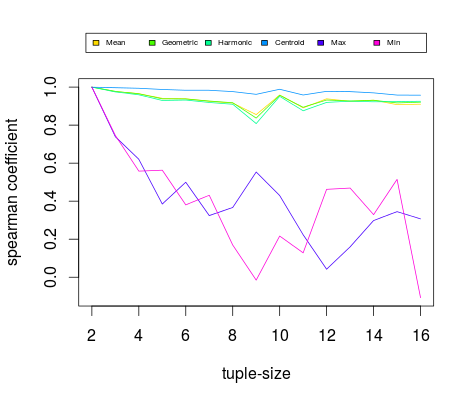
\includegraphics[width=0.5\textwidth]{gfx/correlations/spearman.png}
                \label{fig:5-tuples}
        }
        
        \subfloat[5-tuples with mean euclidean distance to a centroid]{
                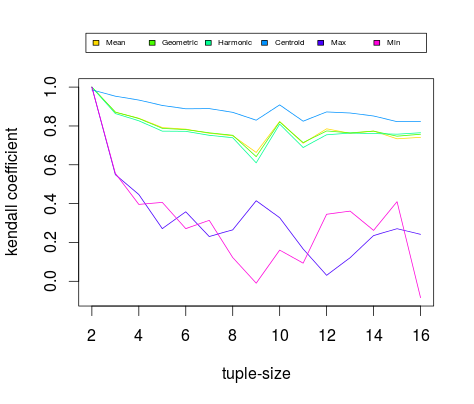
\includegraphics[width=0.5\textwidth]{gfx/correlations/kendall.png}
                \label{fig:5-tuples}
        }

        \caption[Correlation with divergence in 15-dimensional space]{Correlation with divergence in 15-dimensional space}\label{fig:corr-mean}
\end{figure}

%\section{Performance}
%When many calculations are performed over a given metric space, the complexity of individual vectors need only be calculated once and stored for later use, thus amortising the  cost of the calculation when multiple calls to divergence are required. The only calculation required is the complexity of the centroid, followed by some simple arithmetic, making the calculation really quite cheap.
%
%The performance of all the metrics depends on the number of distance calls required: divergence is constant, mean distance to centroid is linear, and mean distance is quadratic. We measured this to see the practical impact, Figure \ref{fig:performance} shows the time in nanoseconds to evaluate each function.  The mean inter-cluster distance is an order of magnitude slower than divergence when the set size is just 5. 

%\begin{figure}
%        \centering
%        \subfloat[Performance vs SED]{
%				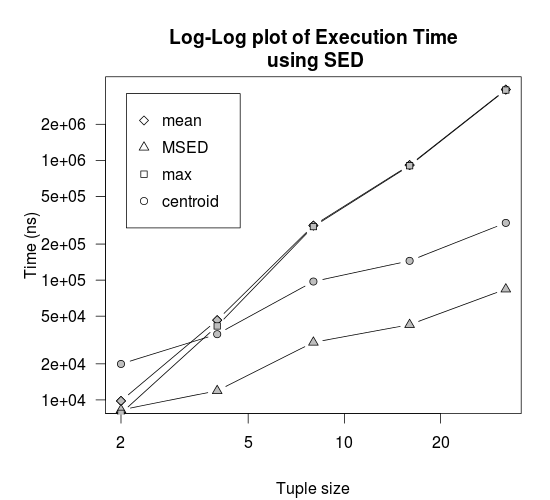
\includegraphics[width=0.5\textwidth]{gfx/sed_times.png}
%                \label{fig:triples}
%        }%
%        ~ %add desired spacing between images, e. g. ~, \quad, \qquad etc.
%          %(or a blank line to force the subfigure onto a new line)
%        \subfloat[Performance vs Euclidean Distance]{
%                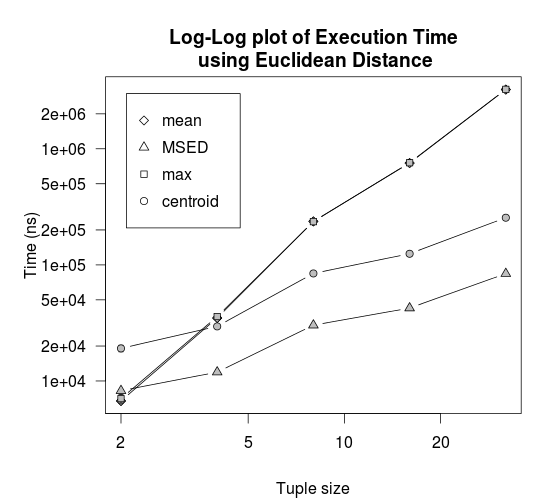
\includegraphics[width=0.5\textwidth]{gfx/euc_times.png}
%                \label{fig:5-tuples}
%        }
%
%        \caption[Performance]{Performance}\label{fig:msed_performance}
%\end{figure}

%We have recently made the observation that the function we had derived as a  distance function $d$ can be logically generalised to a definition over multiple operands; that is, it is a special case of a more general  function $D$ over a set of ensembles, such that $d(e_1,e_2) = D(\{e_1,e_2\})$.
%
%Our original ensemble distance is defined in terms of complexity and merge functions  ($C$ and $M$ respectively) over ensembles as follows:
%\[
%d(e_1,e_2) = \frac{C(M(e_1,e_2))}{\sqrt{C(e_1) \cdot C(e_2)}} - 1
%\]
%%
%The notional merge operator%
%\footnote{the name derives from ensembles used to model structured data}  is  an averaging operation over  ensembles:  $M(e_1,e_2)$ forms a new ensemble, with events drawn from $e_1 \cup e_2$, each assigned the  mean  probability of that event in $e_1$ and $e_2$. The complexity function $C(e)$ is $x^{H_x(e)}$ where $H_x(e)$ is the Shannon entropy \cite{}%
%\footnote{\cite{} gives much deeper mathematical insight of great value in this context} of the ensemble $e$ using base $x$ logarithms.  
%
%Our primary observation is that the semantics underlying the derivation of this form can be generalised to a set $E$ of ensembles, with $n$ elements denoted by $e_i$:
%%
%\[
%D(E) = \left(\frac{C(M'(E))}{\sqrt[n]{ \prod_i {C(e_i) }}} - 1\right) \cdot \frac{1}{n-1}
%\]
%%
%from which  it can be seen how the special case of $n=2$ reverts to the original distance function.
\section{Summary}